\chapter{Regression}
In this section we discuss the datasets we used to research regression.
We will explain in greater detail how our model performed, compare it to other models on and give some info over the dataset.

\section{Used Car Prices}
For this dataset we used the competition version of the big data set provided on Kaggle. This set is based on a big dataset of 100 000 listings on used cars in the UK. We then found and used a version that was slimmed down for competition. This dataset looked ideal for us to learn more about auto-sklearn.
\\
\url{https://www.kaggle.com/adityadesai13/used-car-dataset-ford-and-mercedes?select=vw.csv}
\url{https://www.kaggle.com/kukuroo3/used-car-price-dataset-competition-format}

\subsection{Dataset}

The dataset is based on a list of 100 000 listings of used cars in the UK.
This dataset was preprocessed and separated into competition format.
The label for the test data is provided in the form of a function.
After cleaning the data we where left with the following columns:
\\
carID, brand ,model year, transmission, mileage, fuelType, tax, mpg, engineSize, price.
Their are 2672 entries in total.
\subsection{Model Performance}

First we visualised the dataset with 2 different pairplots.
This gave us an idea of what to expected from this dataset.
The pairplot that is based on the fueltype shows clearly that petrol cars are the most common.
\begin{figure}
    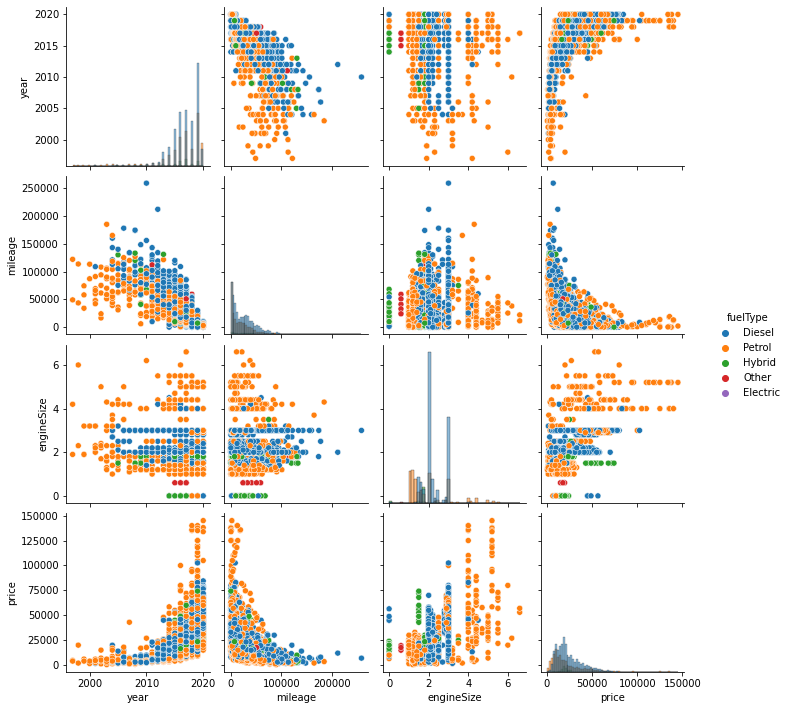
\includegraphics[width=\linewidth]{images/pairplot_fueltype.png}
    \caption{A pairplot based on fueltype}
    \label{fig:pairplot fueltype}
\end{figure}
The pairplot that is based on the brand shows clearly that the german brands are most common.
\begin{figure}
    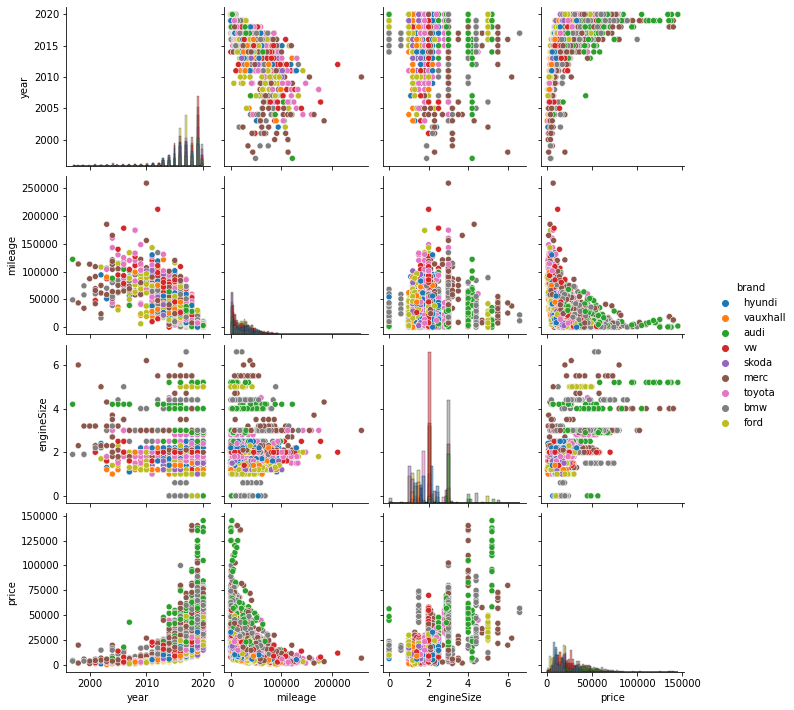
\includegraphics[width=\linewidth]{images/pairplot_brand.png}
    \caption{A pairplot based on brand}
    \label{fig:pairplot brand}
\end{figure}
\\
After fitting and training the data this are the results we got for the different data sets.

\begin{table}[h!]
    \begin{center}
        \caption{Table with training results.}
        \label{tab:training results}
        \begin{tabular}{l|r|r|r} % <-- Changed to S here.
            \textbf{function} & \textbf{Training data} & \textbf{Test data} & \textbf{Test Validation data}\\
            \hline
            mean squared error & 59050.4794 & 293230.5317 & 585230.4846\\
            mean absolute error & 26.3980 & 55.7094 & 59.8129\\
            r2 & 0.9998 & 0.9989 & 0.9979\\
        \end{tabular}
    \end{center}
\end{table}

\subsection{Model Comparision}


\url{https://www.kaggle.com/selinsong/u-car-rf-r2-score-0-94/data}

\url{https://www.kaggle.com/yuyuyuyuy/rf-test-r2-score-0-956}

\url{https://www.kaggle.com/johyunkang/py-rf-test-r2-0-939}

after comparing our work to these 3 projects found on kaggle we can conclude that we are not that far off on performance as the other entries.
\section{Television Brand E-commerce}
\lipsum[2-2]

\subsection{Dataset}
\lipsum[2-2]

\subsection{Model Performance}
\lipsum[2-2]

\subsection{Model Comparision}
\lipsum[2-2]